\chapter{IP伝送装置の性能要件}
\label{chap:network-transmission}

% \section{仮説}
映像のIP伝送については既に多くの先行研究があり、映像を拠点間などで伝送するための製品なども存在している。
しかし、本論文では拠点間のIP伝送だけにとどまらず、拠点内の設備までもをIP伝送する、Video over IPをテーマとしている。

そのため、実際の映像制作現場でIPによる映像伝送を普及させた際に、現在の拠点間のIP伝送が抱える課題を洗い出し、拠点内でも快適にIP伝送を利用することができる要点をまとめ、それが可能であるかについて検証する。

\section{映像制作現場の構成}

現在の映像制作現場には、カメラ、スイッチャー、ディスプレイなどをはじめとする多くの機器がある。
現在の中継現場における、機器同士の接続図を図\ref{fig:broadcast-diagram-on-sdi}に示す。
実際の中継現場では、映像の記録を行うためのレコーダー、映像の入出力を切り替えるためのルーターなどあることが多いが、ここでは割愛する。

\begin{figure}[htbp]
  \begin{center}
    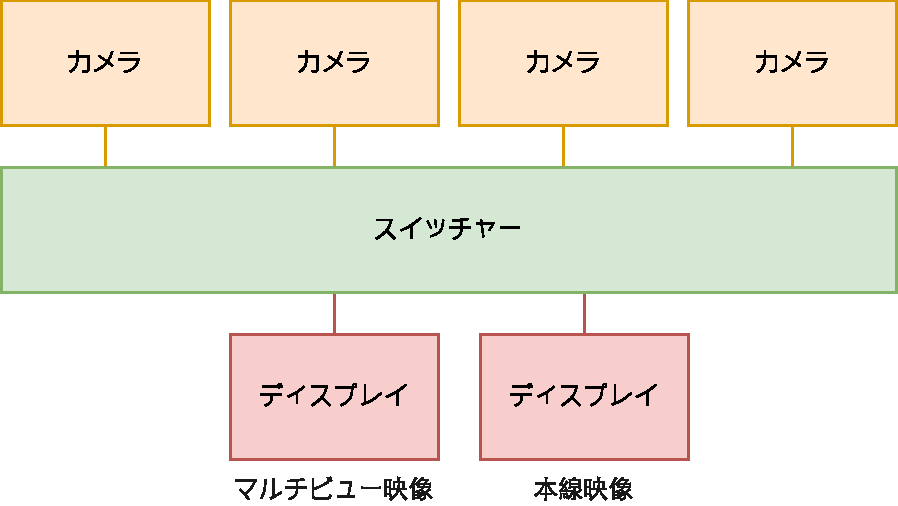
\includegraphics[bb=0 0 432 222,width=8.233cm]{img/broadcast-diagram-on-sdi.pdf}
  \end{center}
  \caption{現在の映像制作現場における機器同士の接続図}
  \label{fig:broadcast-diagram-on-sdi}
\end{figure}

4台のカメラを1台のスイッチャーに入力し、本線映像が出力される。
入力されたソースの映像が複数並んだマルチビュー映像を見てオペレーターが操作することが一般的である。
カメラとスイッチャー、スイッチャーとディスプレイは、それぞれSDIで伝送を行う。

Video over IP化が進んだ将来、理想的な中継現場における機器同士の接続図を図\ref{fig:broadcast-diagram-on-ip}に示す。

\begin{figure}[htbp]
  \begin{center}
    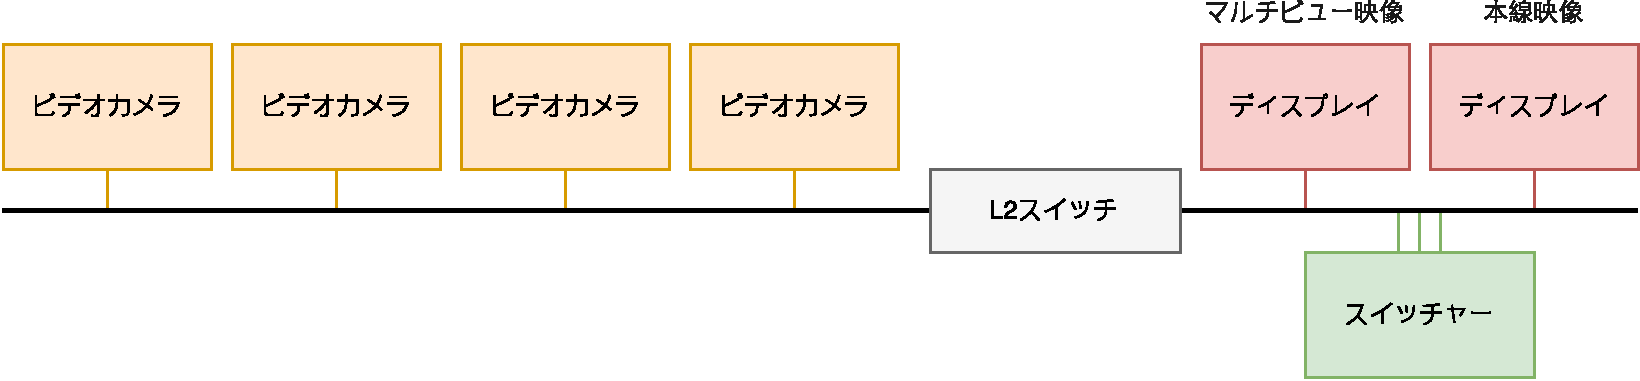
\includegraphics[bb=0 0 787 161,width=15cm]{img/broadcast-diagram-on-ip.pdf}
  \end{center}
  \caption{将来的な映像制作現場における機器同士の接続図}
  \label{fig:broadcast-diagram-on-ip}
\end{figure}

カメラとスイッチャー、スイッチャーとディスプレイは、それぞれIPで伝送を行う。
カメラからスイッチャーには1本の光ファイバーで接続されているが、スイッチャーからはソース映像、本線映像、マルチビュー映像のために3本の光ファイバーで接続されている。
設定解像度の使用する帯域によっては、1本で全ての映像を伝送できる場合もある。

\section{映像制作現場における遅延の許容値の調査}

中継現場で拠点間の映像のIP伝送であれば、ある程度の遅延を許容することができる。
屋外での中継で、外にいるリポーターと局内にいるキャスターとの音声に遅延があり、やり取りに間がある光景を見ることは少なくない。
しかし、拠点内での映像のIP伝送では、映像と音声が同期している必要があり、遅延はシビアな問題となる。

これを実証するために、映像制作現場において、オペーレーターが許容できる遅延の範囲を調査する実験を行った。

\subsection{実験方法}

ブラウザ上で、キーボードの入力を利用した擬似的なスイッチャーの操作を行い、マルチビュー映像の出力を行うプログラムを開発した。音声は出力されない。
プログラムで出力されるマルチビュー映像を図\ref{fig:mv-delay-virtual}に示す。これは、実際の中継現場で利用されているマルチビュー映像とほぼ同じである。

\begin{figure}[htbp]
  \begin{center}
    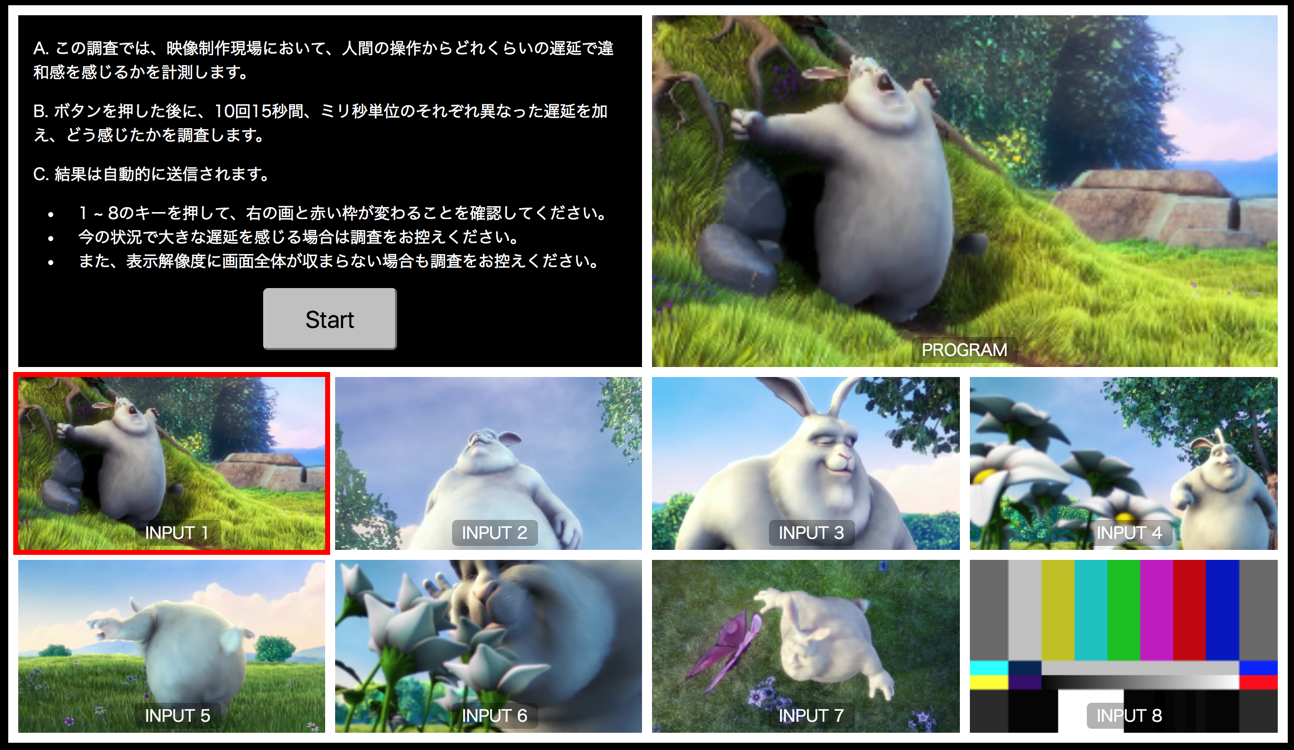
\includegraphics[bb=0 0 1294 750,width=14cm]{img/mv-delay-virtual.png}
  \end{center}
  \caption{今回の実験でWebページ上に再現したマルチビュー映像}
  \label{fig:mv-delay-virtual}
\end{figure}

\begin{figure}[htbp]
  \begin{center}
    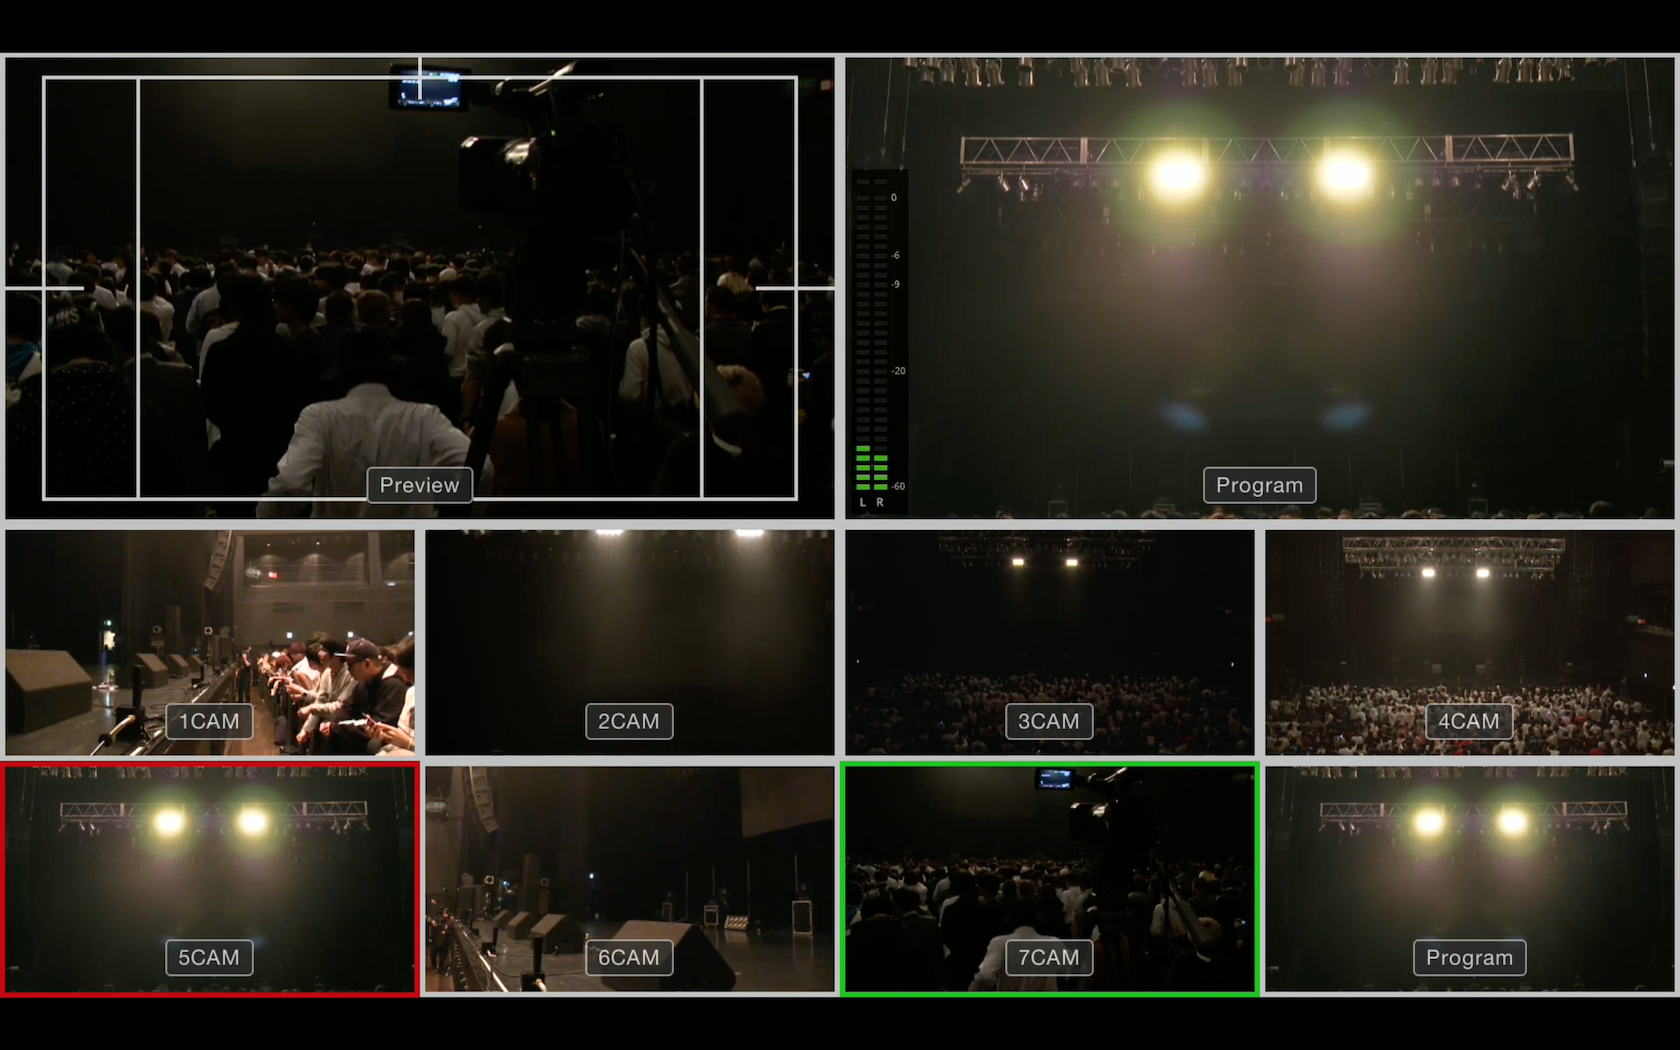
\includegraphics[bb=0 0 1680 1050,width=14cm]{img/mv-delay-actual.png}
  \end{center}
  \caption{実際の中継現場で利用されているマルチビュー映像}
  \label{fig:mv-delay-actual}
\end{figure}

実験では、$0ms$から$499.99ms$までを、1/30秒である$33.33ms$間隔で分けた16段階のステップにわけ、各段階で入力から表示までの遅延を与える。
各段階で与える遅延については、心理的な判断を避けるため実験終了後まで表示を行わない。また、各段階で与える遅延は、実験ごとにランダムになっている。
各段階では、被験者からの入力を15秒間受け付ける。各段階の終了後、被験者に「遅延を許容できる」か「遅延を許容できない」かを問う。

この実験では、図\ref{fig:broadcast-diagram-on-ip}において、スイッチャーとマルチビュー映像を表示するためのディスプレイ間での遅延が許容できるかについて調査したことと同義である。
なお、実験では、ブラウザのレンダリングによる遅延も発生するため、キー入力からブラウザのレンダリングによる遅延も計測した。

被験者の対象は、映像制作現場に関わったことがある人で、マルチビュー映像に理解がある人と限定した。被験者は38人である。

\newpage
\subsection{計測結果}

全被験者からの総入力回数は、10645回であった。キー入力からブラウザのレンダリングによる遅延の平均は、8.6889msであった。
ブラウザのレンダリングによる遅延は、60FPSにおける1フレーム未満であるため、ここでは無視できるものとした。

遅延時間における「遅延を許容できる」と回答した人数を表\ref{tb:mv-delay-result}に示す。

\begin{table}[htbp]
  \caption{映像制作現場における遅延の許容結果}
  \label{tb:mv-delay-result}
  \begin{center}
  \begin{tabular}{r|r}
    \hline
    遅延時間   & 「遅延を許容できる」と回答した人数 \\\hline\hline
    0 ms      & 37 \\\hline
    33.33 ms  & 38 \\\hline
    66.66 ms  & 36 \\\hline
    99.99 ms  & 35 \\\hline
    133.33 ms & 35 \\\hline
    166.66 ms & 31 \\\hline
    199.99 ms & 28 \\\hline
    233.33 ms & 26 \\\hline
    266.66 ms & 18 \\\hline
    299.99 ms & 13 \\\hline
    333.33 ms & 14 \\\hline
    366.66 ms & 15 \\\hline
    399.99 ms & 15 \\\hline
    433.33 ms & 14 \\\hline
    466.66 ms & 13 \\\hline
    499.99 ms & 10 \\\hline
  \end{tabular}\end{center}
\end{table}

\subsection{考察}

映像制作現場における遅延の許容結果のグラフを図\ref{fig:mv-delay-result-graph}に示す。

\begin{figure}[htbp]
  \begin{center}
    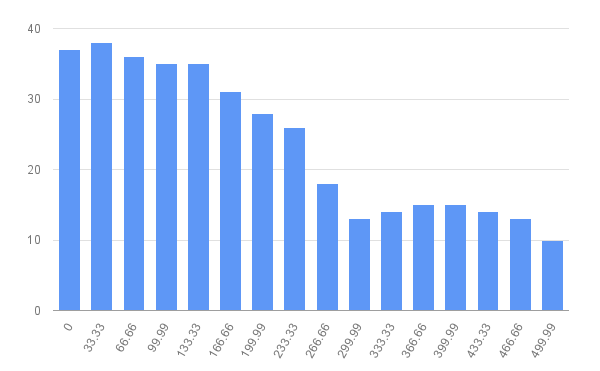
\includegraphics[bb=0 0 600 371,width=13cm]{img/mv-delay-result-graph.png}
  \end{center}
  \caption{映像制作現場における遅延の許容結果のグラフ}
  \label{fig:mv-delay-result-graph}
\end{figure}

133.33msまでの遅延では、被験者の9割以上が「遅延を許容できる」と回答しているが、166.66msの遅延では、8割を下回った。
また、233.33msから266.66msの遅延になると、被験者の過半数が「遅延を許容できない」と回答した。

その他、グラフから読み取れる点として、299.99msから366.66msで人数が多少増加している。
この原因としては、前述の通り各段階で与える遅延の順番はランダムであるため、前段階の遅延よりも短かった場合に体感的に「遅延を許容できる」と回答してしまった人がいるのではいかと考える。

遅くとも133.33msの遅延であれば、9割以上が遅延を許容できるため、過酷な映像制作現場に遅延が許容できると考えられる。
133.33msは、30FPSで4フレーム、60FPSで8フレームである。

\section{まとめ}
本章では、IP伝送装置における性能の要件について調査した。

映像制作現場では、遅延が133.33ms以内であることが望まれる。

\begin{table}[htbp]
  \caption{IP伝送装置の性能要件}
  \label{tb:ip-youken}
  \begin{center}
  \begin{tabular}{l|l}
    \hline
    遅延時間    & 133.33ms以内 \\\hline
    トラフィック & 10Gbps以内 \\\hline
  \end{tabular}\end{center}
\end{table}

% \subsection{Ethernetを活用するメリット}

% \ref{chap:introduction}章で、述べた通り、ネットワークを活用することによって活かせるメリットは以下の3つである。
%
% \begin{itemize}
%   \item 1本のケーブルで複数や双方向の映像が可能
%   \item 伝送スピードの向上
%   \item コストダウン
% \end{itemize}
%
% しかし、Ethernetを利用するためにはデメリットがある
%
% 輻輳
% 導入コストの
%
% また、映像伝送における重要なポイントは以下の3つである。
%
% \begin{itemize}
%   \item 画質、音質の劣化がない
%   \item 伝送遅延を一定以下にする必要がある
%   \item 安定性がある
% \end{itemize}
%
% また、IP伝送のメリットは以下の点である。
%
% \begin{itemize}
%   \item ユニキャスト、ブロードキャストが行える
% \end{itemize}
%
% これらの点において評価を行う。

% \section{映像制作現場で求められるIP伝送の要件}
% % ファイルベースの映像編集では、ネットワークストレージを活用した環境
% % しかし、ライブでは、同軸ケーブルを利用してきました。これは、映像や音声を安定的に伝送することが求められているからです。
%
% リアルタイムの映像伝送では、前出の通り同軸ケーブルを使用することが一般的である。
%
% 映像や音声を安定的に伝送することが出来、
% 現場での取り回しの氏易さ
% IP
%
% % \section{遅延}
%
% \section{NG-HDMI-TSの目的}
%
% 映像制作の現場では、符号化・複合などによる映像の遅延を抑えることや、画質をそのまま伝送することがしばしば求められます。
% このような背景から、4K映像を非圧縮のままIP伝送する技術の実証実験と、現場においてIP伝送を利用する際に問題となる点を洗い出します。?

% \section{構成}
